\section {Introduction to DFA Framework}
\setlength{\parindent}{0pt}
(Prepared by Namrata Priyadarshani and Shivam Bansal)

\vspace{0.3cm}

In this module, we build up common framework to express DFA. Some common characteristics of DFA are described below: 

\subsection{Transfer Functions and Meet operator}

Let s be a statement and the value before statement is in[s] and after statement is out[s]. Then, for a forward DFA, \textbf{Transfer function} is defined as the function that takes in[s] as argument and converts it into out[s]. \textbf{Meet operator} expresses in[s] as the function of out[p] for all predecessor p of s. These functions operates in reverse direction in the case of Backward DFA.
\newline
Most of the time, we consider running the algorithm at the Basic Block level granularity and define Transfer function and meet operator for the values in[B] and out[B] i.e. the input and output values of the basic block B. 

\subsection{Partial ordered values}

There is a partial order within the elements of Domain represented by $\geq$ operator.
Directed Acyclic Graph is one way to represent the ordering. The graph contains an edge from $a \rightarrow b$ iff $a \geq b$.
%insert image
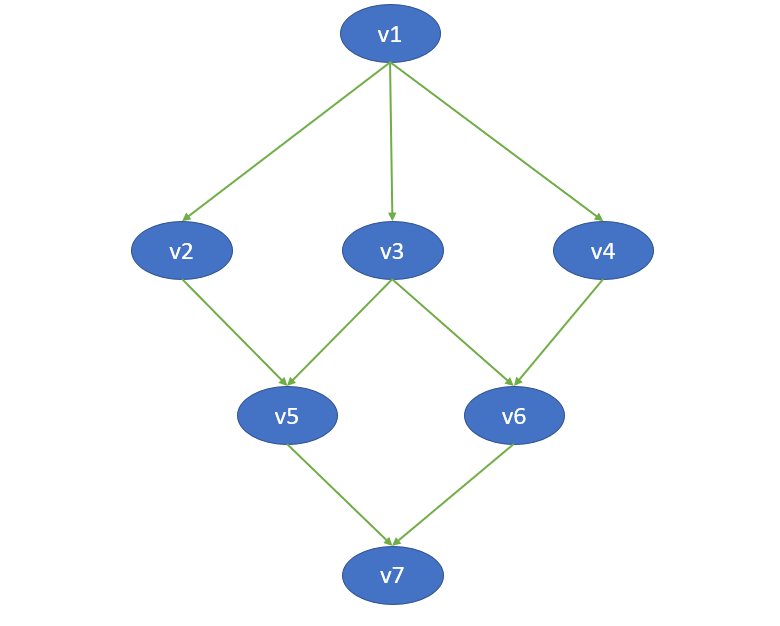
\includegraphics[scale=0.3]{images/91_1.png}
There is one value greater than all values in Domain known as Top value (T) and one value less than all values in Domain known as Bottom value ($ \bot $).

\subsection{Constant Propagation DFA}
Different DFA has different direction, boundary condition, meet operator and transfer function. The structure and flow of algorithm remains same for all DFA. In fixed-point-algorithm first the boundary condition is specified, all other values are set to top value and then iterate until no change occur in any value.

For constant propagation the DFA is specified by:
\begin{itemize}
    \item \textbf{Domain}: set of constant definitions
    \item \textbf{Direction}: Forward
    \item \textbf{Transfer function}: $f_{B} = \lambda x. GEN[B] \cup (x-KILL[B]) $
    \item \textbf{Meet operator}: $\cap$ (set intersection)
    \item \textbf{Boundary condition}: $out[entry] = \phi$
\end{itemize}
